% !TEX TS-program = xelatex
% !BIB program = bibtex
% !TeX spellcheck = ru_RU
% !TEX root = 02_talk.tex

\documentclass
  [ russian
  , aspectratio=169 % Для защит онлайн лучше использовать разрешение не 4х3
  ] {beamer}


% !TeX spellcheck = ru_RU
% !TEX root = vkr.tex

% Опциональные добавления используемых пакетов. Вполне может быть, что они вам не понадобятся, но в шаблоне приведены примеры их использования.
\usepackage{tikz} % Мощный пакет для создание рисунков, однако может очень сильно замедлять компиляцию
\usetikzlibrary{decorations.pathreplacing,calc,shapes,positioning,tikzmark}

% Библиотека для TikZ, которая генерирует отдельные файлы для каждого рисунка
% Позволяет ускорить компиляцию, однако имеет свои ограничения
% Например, ломает пример выделения кода в листинге из шаблона
% \usetikzlibrary{external}
% \tikzexternalize[prefix=figures/]

\newcounter{tmkcount}

\tikzset{
    use tikzmark/.style={
            remember picture,
            overlay,
            execute at end picture={
                    \stepcounter{tmkcount}
                },
        },
    tikzmark suffix={-\thetmkcount}
}


%% Таблицы
\usepackage{tabularx}
\usepackage{makecell}
\usepackage{booktabs}
\usepackage{multirow}
\usepackage{multicol}
\usepackage{ltablex}
\usepackage{longtable}
\usepackage{array}


% Для названий стоит использовать \textsc{}
\newcommand{\OCaml}{\textsc{OCaml}}
\definecolor{eclipseGreen}{RGB}{63,127,95}

\makeatletter

%%% Обязательные пакеты
%% Beamer
\usepackage{beamerthemesplit}
\usetheme{SPbGU}
\beamertemplatenavigationsymbolsempty
\usepackage{appendixnumberbeamer}

%% Локализация
\usepackage{fontspec}
\setmainfont{CMU Serif}
\setsansfont{CMU Sans Serif}
\setmonofont{CMU Typewriter Text}
% \setmonofont{Fira Code}[Contextuals=Alternate,Scale=0.9]
% \setmonofont{Inconsolata}

\newfontfamily\cyrscfont{Inconsolata}[
  SmallCapsFeatures={Letters=SmallCaps},
  Scale=MatchLowercase
]
\DeclareRobustCommand{\textsc}[1]{{\cyrscfont\addfontfeatures{Letters=SmallCaps}#1}}

\usepackage{polyglossia}
\setmainlanguage{russian}
\setotherlanguage{english}

%% Графика
\usepackage{pdfpages} % Позволяет вставлять многостраничные pdf документы в текст
\usepackage{fancyvrb}

\makeatother

\usepackage[autostyle]{csquotes} % Правильные кавычки в зависимости от языка
\usepackage{totcount}
\usepackage{setspace}
\usepackage{amsmath, amsfonts, amssymb, amsthm, mathtools} % "Адекватная" работа с математикой в LaTeX

\usepackage[labelsep=period,            % вместо ':' ставить '.'
            justification=centering,
            singlelinecheck=false
           ]{caption} % Настройка подписей "не текста"
\usepackage{subcaption} % Подписи для разделенного "не текста"
\addto\captionsrussian{\renewcommand{\figurename}{Рисунок}}

\usepackage{pgf}
\usepackage{colortbl}
\usepackage[table]{xcolor}
\usepackage{highlight}
\definecolor{low}{HTML}{ef3b2c}
\definecolor{mid}{HTML}{fff7f7}
\definecolor{high}{HTML}{66FF66}
\newcommand{\g}[1]{\gradientcelld{#1}{6}{10.5}{11.5}{low}{mid}{high}{70}}
\newcommand{\gr}[1]{\gradientcelld{#1}{2.0}{2.1}{2.8}{high}{mid}{low}{70}}

\newcommand{\h}[1]{%
  \pgfmathparse{#1>0.05}%
  \ifnum\pgfmathresult=1
    \cellcolor{high!50}#1%
  \else
    #1%
  \fi
}

\makeatletter

% !TeX spellcheck = ru_RU
% !TEX root = vkr.tex

%% Параметры заполнения титульного листа
\usepackage{xkeyval}

%% Русскоязычный вариант
\define@key[ru]{mytitle}{chair}{\def\my@title@chair@ru{#1}}
\define@key[ru]{mytitle}{title}{\def\my@title@title@ru{#1}}
\define@key[ru]{mytitle}{group}{\def\my@title@group@ru{#1}}
\define@key[ru]{mytitle}{author}{\def\my@title@author@ru{#1}}
\define@key[ru]{mytitle}{supervisor}{\def\my@title@supervisor@ru{#1}}
\define@key[ru]{mytitle}{supervisorPosition}{\def\my@title@supervisorPosition@ru{#1}}
\define@key[ru]{mytitle}{reviewer}{\def\my@title@reviewer@ru{#1}}
\define@key[ru]{mytitle}{reviewerPosition}{\def\my@title@reviewerPosition@ru{#1}}
\define@key[ru]{mytitle}{consultant}{\def\my@title@consultant@ru{#1}}
\define@key[ru]{mytitle}{consultantPosition}{\def\my@title@consultantPosition@ru{#1}}
\define@key[ru]{mytitle}{year}{\def\my@title@year@ru{#1}}
\define@key[ru]{mytitle}{specialty}{\def\my@title@specialty@ru{#1}}
\define@key[ru]{mytitle}{programme}{\def\my@title@programme@ru{#1}}
\define@key[ru]{mytitle}{profile}{\def\my@title@profile@ru{#1}}
\define@choicekey*[ru]{mytitle}{type}{coursework,practice,prediploma,master,bachelor,production}{\def\my@title@type@ru{#1}}
\define@choicekey*[ru]{mytitle}{kind}{solution,experiment,production,comparison,theoretical}{\def\my@title@kind@ru{#1}}

%% Англоязычный вариант
\define@key[en]{mytitle}{chair}{\def\my@title@chair@en{#1}}
\define@key[en]{mytitle}{title}{\def\my@title@title@en{#1}}
\define@key[en]{mytitle}{group}{\def\my@title@group@en{#1}}
\define@key[en]{mytitle}{author}{\def\my@title@author@en{#1}}
\define@key[en]{mytitle}{supervisor}{\def\my@title@supervisor@en{#1}}
\define@key[en]{mytitle}{supervisorPosition}{\def\my@title@supervisorPosition@en{#1}}
\define@key[en]{mytitle}{reviewer}{\def\my@title@reviewer@en{#1}}
\define@key[en]{mytitle}{reviewerPosition}{\def\my@title@reviewerPosition@en{#1}}
\define@key[en]{mytitle}{consultant}{\def\my@title@consultant@en{#1}}
\define@key[en]{mytitle}{consultantPosition}{\def\my@title@consultantPosition@en{#1}}
\define@key[en]{mytitle}{year}{\def\my@title@year@en{#1}}
\define@key[en]{mytitle}{specialty}{\def\my@title@specialty@en{#1}}
\define@key[en]{mytitle}{programme}{\def\my@title@programme@en{#1}}
\define@key[en]{mytitle}{profile}{\def\my@title@profile@en{#1}}
\define@choicekey*[en]{mytitle}{type}{coursework,practice,prediploma,master,bachelor}{\def\my@title@type@en{#1}}
\define@choicekey*[en]{mytitle}{kind}{solution,experiment,production,comparison,theoretical}{\def\my@title@kind@en{#1}}

\newcommand{\filltitle}[2]{
    %% Значения по умолчанию для обоих языков
    \ifthenelse{\equal{#1}{ru}}
    {
        \presetkeys[#1]{mytitle}{
            year = {\the\year},
            type = {practice},
            reviewer = {},
            consultant = {},
            profile = {}
        }{}
    }
    {}
    \ifthenelse{\equal{#1}{en}}
    {
        \presetkeys[#1]{mytitle}{
            year = {\the\year},
            type = {practice},
            reviewer = {},
            consultant = {},
            profile = {}
        }{}
    }
    {}
    \setkeys[#1]{mytitle}{#2}
}


%% Если что-то забыли, при компиляции будут ошибки Undefined control sequence \my@title@<что забыли>@ru
%% Если англоязычная титульная страница не нужна, то ее можно просто удалить.
\filltitle{ru}{
    %% Актуально только для курсовых/практик. ВКР защищаются не на кафедре а в ГЭК по направлению,
    %%   и к моменту защиты вы будете уже не в группе.
    chair              = {Кафедра информатики},
    %
    %% Макрос filltitle ненавидит пустые строки, поэтому обязателен хотя бы символ комментария на строке
    %% Актуально всем.
    title              = {Определение кода Голланда по результатам психометрических тестов личности на основе методов машинного обучения в условиях неполноты информации},
    %
    %% Здесь указывается тип работы. Возможные значения:
    %%   production - производственная практика;
    %%   coursework - отчёт по курсовой работе (ОБРАТИТЕ ВНИМАНИЕ, у техпрога и ПИ нет курсовых, только практики);
    %%   practice - отчёт по учебной практике;
    %%   prediploma - отчёт по преддипломной практике;
    %%   master - ВКР магистра;
    %%   bachelor - ВКР бакалавра.
    type               = {master},
    %
    %% Здесь указывается вид работы. От вида работы зависят критерии оценивания.
    %%   solution - «Решение». Обучающемуся поручили найти способ решения проблемы в области разработки программного обеспечения или теоретической информатики с учётом набора ограничений.
    %%   experiment - «Эксперимент». Обучающемуся поручили изучить возможности, достоинства и недостатки новой технологии, платформы, языка и т. д. на примере какой-то задачи.
    %%   production - «Производственное задание». Автору поручили реализовать потенциально полезное программное обеспечение.
    %%   comparison - «Сравнение». Обучающемуся поручили сравнить несколько существующих продуктов и/или подходов.
    %%   theoretical - «Теоретическое исследование». Автору поручили доказать какое-то утверждение, исследовать свойства алгоритма и т.п., при этом не требуя написания кода.
    kind               = {solution},
    %
    author             = {ГЛУШКОВ Егор Александрович},
    %
    %% Актуально только для ВКР. Указывается код и название направления подготовки. Типичные примеры:
    %%   02.03.03 \enquote{Математическое обеспечение и администрирование информационных систем}
    %%   02.04.03 \enquote{Математическое обеспечение и администрирование информационных систем}
    %%   09.03.04 \enquote{Программная инженерия}
    %%   09.04.04 \enquote{Программная инженерия}
    %% Те, что с 03 в середине --- бакалавриат, с 04 --- магистратура.
    specialty          = {02.04.03 \enquote{Математическое обеспечение и администрирование информационных систем}},
    %
    %% Актуально только для ВКР. Указывается шифр и название образовательной программы. Типичные примеры:
    %%   СВ.5162.2020 \enquote{Технологии программирования}
    %%   СВ.5080.2020 \enquote{Программная инженерия}
    %%   ВМ.5665.2022 \enquote{Математическое обеспечение и администрирование информационных систем}
    %%   ВМ.5666.2022 \enquote{Программная инженерия}
    %% Шифр и название программы можно посмотреть в учебном плане, по которому вы учитесь.
    %% СВ.* --- бакалавриат, ВМ.* --- магистратура. В конце --- год поступления (не обязательно ваш, если вы были в академе/вылетали).
    programme          = {ВМ.5665.2023 \enquote{Математическое обеспечение и администрирование информационных систем}},
    %
    %% Актуально всем.
    %% Должно умещаться в одну строчку, допускается использование сокращений, но без переусердствования,
    %% короткая строка с большим количеством сокращений выглядит странно
    %supervisorPosition = {проф. кафeдры системного программирования, д.ф.-м.н.,}, % Терехов А. Н.
    %supervisorPosition = {ст. преподаватель кафедры ИАС, к.~ф.-м.~н. (если есть),}, % Смирнов К. К.
    supervisorPosition = {доцент кафедры информатики, к.~т.~н.,},
    supervisor         = {Абрамов~М.~В.},
    %
    %% Актуально только для практик и курсовых. Если консультанта нет или он совпадает с научником, закомментировать или удалить вовсе.
    consultantPosition = {ст. преподаватель кафедры информатики,},
    consultant         = {Столярова~В.~Ф.},
    %
    %% Актуально только для ВКР.
    reviewerPosition   = {ст. научный сотрудник, СПб~ФИЦ~РАН, к.~т.~н.,},
    reviewer           = {Захаров~В.~В.},
}

% Английский титульник нужен только для ВКР, остальные виды работ могут его смело игнорировать.
\filltitle{en}{
    chair              = {Advisor's chair},
    title              = {Determination of the Holland Code based оn the results of psychometric personality tests using machine learning methods in the presence of incomplete information},
    type               = {master},
    author             = {Egor Glushkov},
    %
    %% Possible choices:
    %%   02.03.03 \foreignquote{english}{Software and Administration of Information Systems}
    %%   02.04.03 \foreignquote{english}{Software and Administration of Information Systems}
    %%   09.03.04 \foreignquote{english}{Software Engineering}
    %%   09.04.04 \foreignquote{english}{Software Engineering}
    %% Те, что с 03 в середине --- бакалавриат, с 04 --- магистратура.
    specialty          = {02.04.03 \foreignquote{english}{Software and Administration of Information Systems}},
    %
    %% Possible choices:
    %%   СВ.5162.2020 \foreignquote{english}{Programming Technologies}
    %%   СВ.5080.2020 \foreignquote{english}{Software Engineering}
    %%   ВМ.5665.2022 \foreignquote{english}{Software and Administration of Information Systems}
    %%   ВМ.5666.2022 \foreignquote{english}{Software Engineering}
    programme          = {ВМ.5665.2023 \foreignquote{english}{Software and Administration of Information Systems}},
    %
    %% Note that common title translations are:
    %%   кандидат наук --- C.Sc. (NOT Ph.D.)
    %%   доктор ... наук --- Sc.D.
    %%   доцент --- docent (NOT assistant/associate prof.)
    %%   профессор --- prof.
    supervisorPosition = {C.Sc., docent, Department of CS,},
    supervisor         = {M.~V.~Abramov},
    %
    consultantPosition = {senior lecturer, Department of CS,},
    consultant         = {V.~F.~Stoliarova},
    %
    reviewerPosition   = {C.Sc., senior researcher, SPb FRC RAS,},
    reviewer           = {V.~V.~Zakharov},
}


\newcommand{\advisorChair}{\my@title@chair@ru}
% То, что в квадратных скобках, отображается внизу по центру каждого слайда.
\title[Определение кода Голланда]{\my@title@title@ru}
% То, что в квадратных скобках, отображается в левом нижнем углу.
\author[\my@title@author@ru]{\my@title@author@ru}
\institute[СПбГУ]{}
\date[14 июня 2025 г.]{}
\newcommand{\supervisor}{\my@title@supervisor@ru}
\newcommand{\supervisorPosition}{\my@title@supervisorPosition@ru}
\newcommand{\consultant}{\my@title@consultant@ru}
\newcommand{\consultantPosition}{\my@title@consultantPosition@ru}
\newcommand{\reviewer}{\my@title@reviewer@ru}
\newcommand{\reviewerPosition}{\my@title@reviewerPosition@ru}
\newcommand{\defenseYear}{\my@title@year@ru}

\makeatother
\begin{document}
{
\setbeamertemplate{footline}{}
% Лого университета или организации, отображается в шапке титульного листа
\begin{frame}
    
\includegraphics[width=1.4cm]{figures/SPbGU_Logo.png}
    \vspace{-30pt}
    \hspace{-10pt}
    \begin{center}
        \begin{tabular}{c}
            \small{Санкт-Петербургский государственный университет} \\
            \small{\advisorChair}
        \end{tabular}
        \titlepage
        \vspace{-3em}
    \end{center}

    {\small
        \textbf{Научный руководитель:}  \supervisorPosition~\supervisor \\
        \textbf{Консультант:}  \consultantPosition~\consultant \\
        \textbf{Рецензент:} \reviewerPosition~\reviewer \\
    }
    \makeatother
    \vspace{1.5em}
    
    \begin{center}
        \small{Санкт-Петербург, \defenseYear}
    \end{center}
\end{frame}
}


\begin{frame}
    \frametitle{Введение}
    \begin{itemize}
        \item Важность корректного выбора профессионального пути

        \vspace{4pt}
        \item Ресурсоёмкость традиционного глубинного интервью, дистанционные методы профориентации, психометрические тесты

        \vspace{4pt}
        \item Модель RIASEC (код Голланда): 
            \begin{itemize}
                \item шесть типов социально-профессиональной направленности личности
                \item различные вариации теста
                \item сравнение профессиональных профилей с помощью C-индекса
            \end{itemize}

        \vspace{4pt}
        \item Взаимосвязь кода Голланда с социально-демографическими признаками, цифровыми следами, психометрическими тестами с помощью статистических методов, структурного моделирования, машинного обучения

        \vspace{4pt}
        \item Нет инструментов, позволяющих по комбинации популярных тестов предсказывать код Голланда, особенно в условиях неполноты информации
    \end{itemize}
\end{frame}


\begin{frame}
    \frametitle{Постановка задачи}
    \textbf{Целью} работы является автоматизация процесса профориентации посредством разработки инструмента для предсказания кода Голланда по неполным результатам психометрических тестов с использованием методов машинного обучения
    \vspace{0.5em}

    \textbf{Задачи}:
    \begin{itemize}
        \item Реализовать различные подходы к определению кода Голланда: многоцелевая регрессия, классификация, ранжирование
        \item Разработать модуль формирования взвешенного ансамбля моделей для объединения прогнозов базовых моделей
        \item Провести сравнительный анализ подходов и методов определения кода Голланда на основе C-индекса
        \item Разработать математическое обеспечение для модуля восстановления пропусков психометрических тестов
        \item Создать прототип инструмента для определения профориентационных предпочтений 
    \end{itemize}
\end{frame}


\begin{frame}
    \frametitle{Новизна и значимость}
    \begin{itemize}
        \item \emph{Новизна результатов исследования}: создание нового программного комплекса, обеспечивающего автоматизацию процесса профориентации на основе предсказания кода Голланда
        \vspace{0.6em}
        \item \emph{Теоретическая значимость}: использование уникальной комбинации различных психометрических тестов при разработке новых моделей машинного обучения для определения взаимосвязи тестов и кода Голланда
        \vspace{0.6em}
        \item \emph{Практическая значимость}: разработка прототипа программного модуля автоматизации оценки профессиональной направленности по психологическому профилю личности
    \end{itemize}
\end{frame}


\begin{frame}
    \frametitle{Обзор. Психометрические  тесты личности}
    {
    \setlength{\leftmargini}{3em}
    \begin{itemize}
        \item Тест Голланда RIASEC (6)\\
         {\footnotesize 6 типов (профилей) личностей, с которыми соотнесены наборы профессий}
        \item Опросник Леонгарда-Шмишека (10)
        \item Личностный опросник Айзенка (4)
        \item 16-факторный опросник Кеттелла (16)
        \item Пятифакторный опросник личности («Большая пятерка»; 5)
        \item Ценностный опросник Шварца (20)
    \end{itemize}
    }
        
    \setlength{\abovecaptionskip}{3pt}
    \setlength{\belowcaptionskip}{1.5pt}
    \begin{table}
      \centering
      \footnotesize
      \caption{Пример данных психометрических тестов}
      \label{tab:input_test_data}
      \begin{tabular}{
        >{\centering\arraybackslash}p{0.45cm}       |  % id
        *{3}{>{\centering\arraybackslash}p{0.6cm}}     % BF
        >{\centering\arraybackslash}p{0.165cm}         % ...
        *{2}{>{\centering\arraybackslash}p{0.66cm}} |  % LN
        *{6}{>{\centering\arraybackslash}p{0.5cm}}     % HL
      }
        \toprule
        \multirow{2}{*}{\textbf{id}}
          & \multicolumn{3}{c}{\textbf{Большая пятёрка}}
          & \multirow{2}{*}{\textbf{\dots}}
          & \multicolumn{2}{c|}{\textbf{Леонгард}}
          & \multicolumn{6}{c}{\textbf{Голланд}} \\
        \cmidrule(lr){2-4} \cmidrule(lr){6-7} \cmidrule(lr){8-13}
          & BF1 & BF2 & BF3 
          & 
          & LN9 & LN10 
          & R & I & A & S & E & C \\
        \midrule
        1 & 39 & 66 & 33 & \dots &  3 & 12  &  8 &  8 &  6 &  8 &  1 & 11 \\
        2 & 45 & 46 & 73 & \dots & 12 &  6  &  3 &  7 &  7 &  8 & 10 &  7 \\
        3 & 34 & 41 & 56 & \dots & 18 & 12  & 10 & 10 &  3 & 11 &  7 &  1 \\
        4 & 49 & 47 & 50 & \dots & 15 & 24  &  6 &  4 &  8 &  6 &  7 & 11 \\
        \bottomrule
      \end{tabular}
    \end{table}
\end{frame}


\begin{frame}
    \frametitle{Общая схема вариантов вычислительного эксперимента}
    \begin{figure}
        \centering
        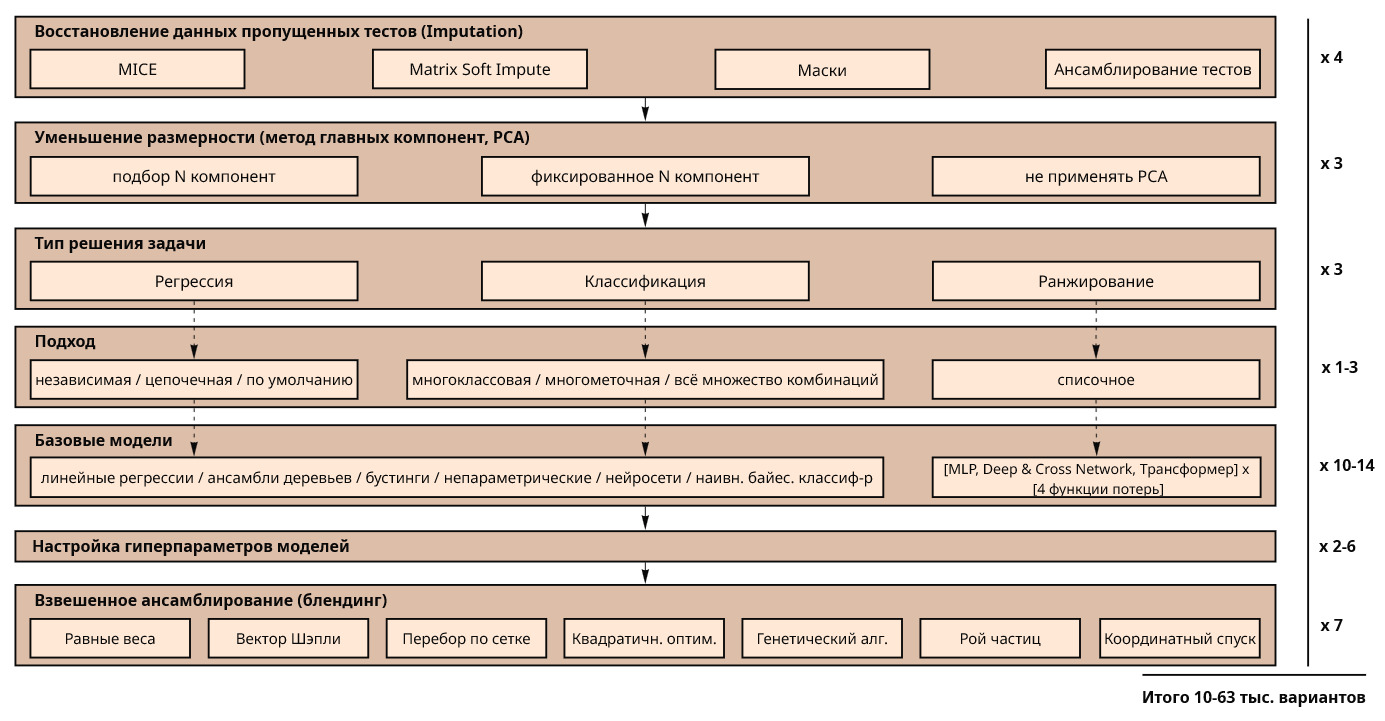
\includegraphics[width=0.9\linewidth]{figures/multi_pipeline.jpg}
        \vspace{-0.9em}
        \captionsetup{font=footnotesize}
        \caption{Общая схема вариантов вычислительного эксперимента}
        \label{fig:multi_pipeline}
    \end{figure}
\end{frame}


\begin{frame}
    \frametitle{Подходы и метрики качества}
    \begin{itemize}
        \item Многоцелевая регрессия~--- метрика \emph{avgRMSE}
        \item Классификация~--- \emph{Top-k accuracy}
        % \vspace{0.4em}
        \item Ранжирование~--- \emph{NDCG@3}
    \vspace{0.6em}
    \item Сравнение подходов на основе C-индекса, желаемое значение: $C_\text{index} \geq 11$
  \[
    C_\text{index} = 3\, (X_1, Y_1) + 2\, (X_2, Y_2) + 1\, (X_3, Y_3),
  \]
  где $\{X_i\}$ и $\{Y_i\}$ — первые три позиции кодов Голланда, их позиции в замкнутой цепочке (шестиугольнике) \textit{R-I-A-S-E-C}:
  \[
    (X_i, Y_i) =
    \begin{cases}
      3, & \text{если $X_i = Y_i$,}\\
      2, & \text{если $X_i$ и $Y_i$ -- соседние позиции,}\\
      1, & \text{если $X_i$ и $Y_i$ -- позиции через один код,}\\
      0, & \text{если $X_i$ и $Y_i$ -- противоположны.}
    \end{cases}
  \]
  \end{itemize}
\end{frame}


\begin{frame}
    \frametitle{Особенности реализации}
    \begin{itemize}
        \item R (версия 4.4.2):
        \begin{itemize}
            \item векторизованная обработка и манипуляции с данными: \textit{data.table, tidyverse, R6}
            \item статистические и ML-модели: \textit{stats, mice, softImpute, glmnet, MASS, xgboost, lightgbm, catboost, randomForest, FNN, caret, e1071, ranger, quadprog, GA, PSO}
            \item интерактивные веб-приложения: \textit{Shiny (Posit)}; визуализация: \textit{plotly}
        \end{itemize}
        
        \vspace{0.2em}
        \item Python (версия 3.12.3):
        \begin{itemize}
            \item \textit{numpy, pandas, sklearn, PyTorch, TabPFN}
        \end{itemize}

        \vspace{0.2em}
        \item Основные этапы реализации\textsuperscript{1}:
        \begin{enumerate}
            \item Разведочный анализ данных
            \item Вычислительный эксперимент: выбор наилучшего подхода к определению кода Голланда, обучение и сохранение модели
            \item Прототип инструмента автоматизации профориентации (веб-приложение) 
        \end{enumerate}
    \end{itemize}
    
    \btVFill
    {\footnotesize
        \textsuperscript{1} GitHub: Предсказание кода Голланда (RIASEC) по результатам психометрических тестов личности.\\
        \quad URL: \url{https://github.com/ExP98/Diploma_Holland} (дата обращения: 07.06.2025)
    }
\end{frame}


\begin{frame}
    \frametitle{Архитектура вычислительного модуля}
    \begin{figure}
        \centering
        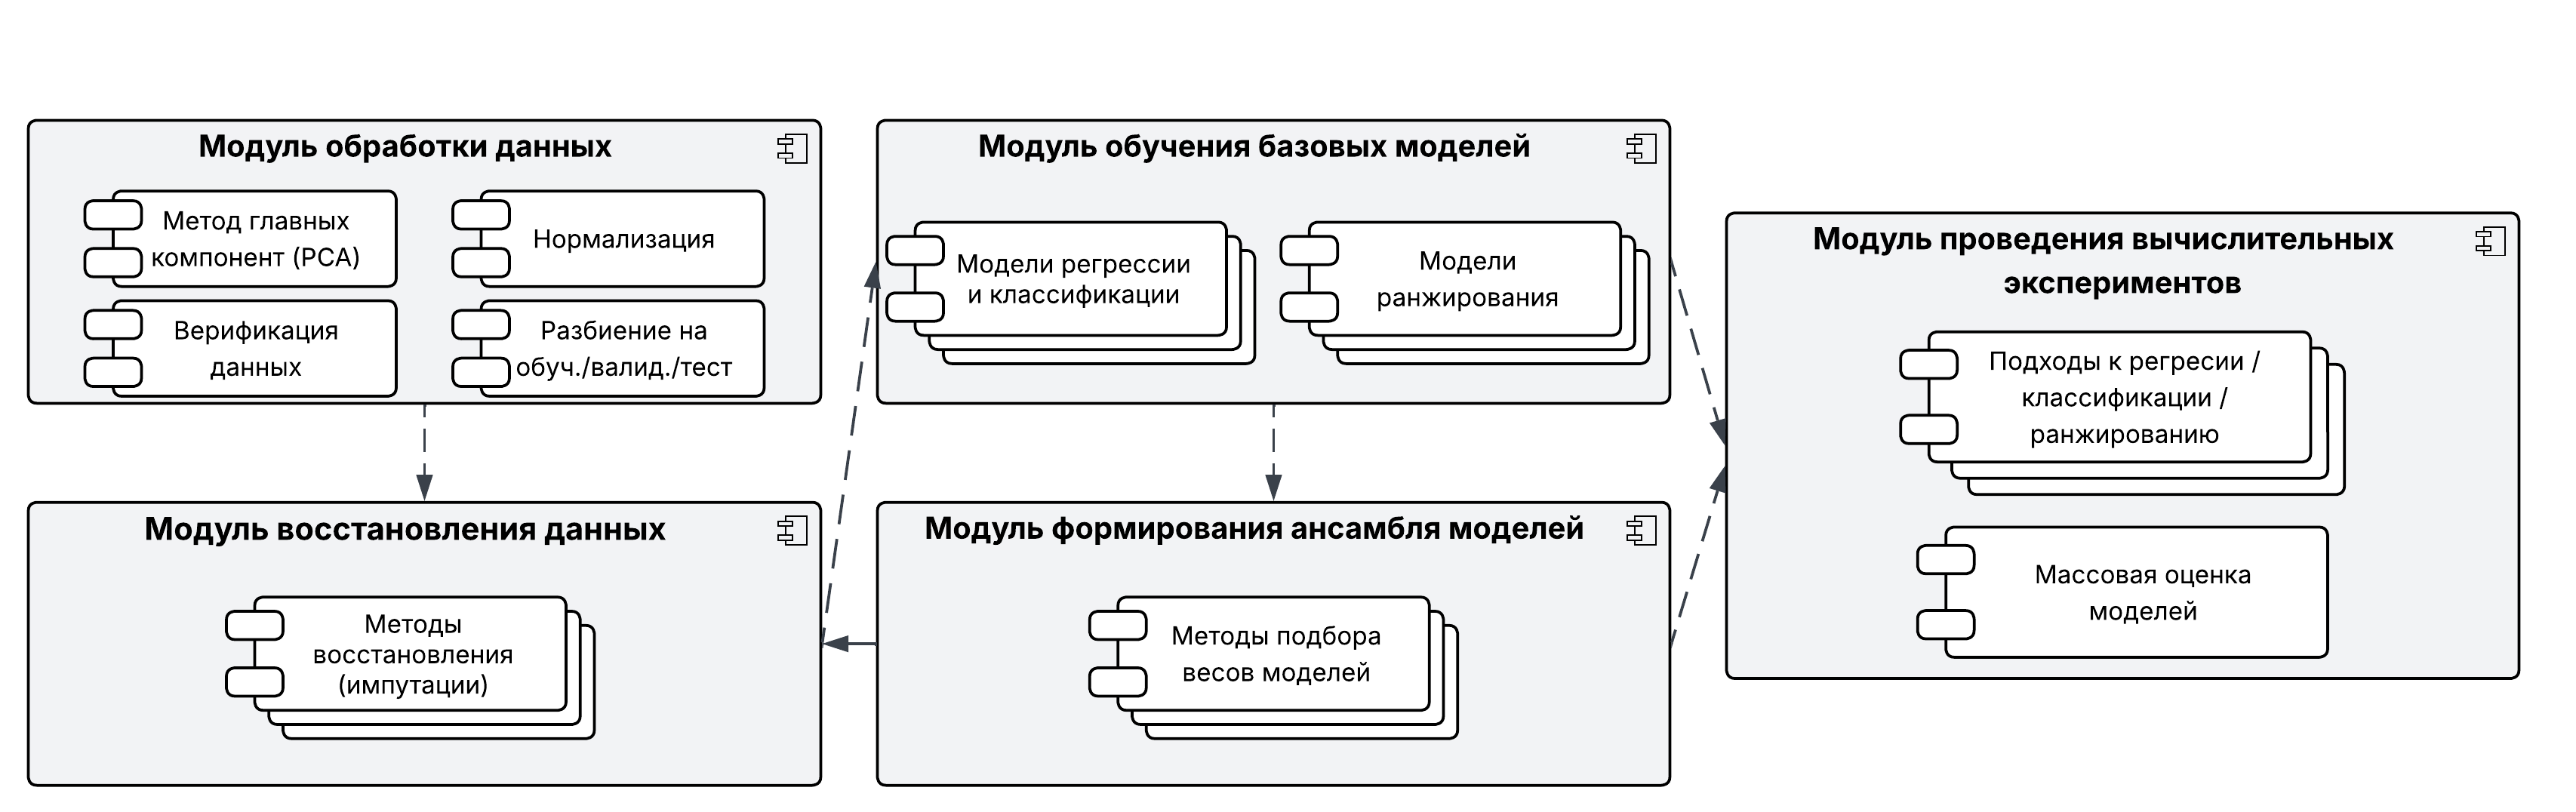
\includegraphics[width=1\linewidth]{figures/Arch_colored.png}
        \caption{Архитектура вычислительного модуля}
        \label{fig:archi}
    \end{figure}
\end{frame}


\begin{frame}
    \frametitle{Описание набора данных}
    \begin{columns}[T]
    \begin{column}{0.48\textwidth}
        \small
        \begin{itemize}
            \item VK Mini Apps «Психологические тесты»\textsuperscript{2}
            \item Анонимизированные данные\textsuperscript{3} 1278 пользователей: 339~--- полные, 939~--- не заполнены данные по 1--2 тестам
            \item Обработка данных: json $\rightarrow$ широкий табличный формат, валидация, заполнение пропусков, нормализация, понижение размерности (метод главных компонент, \emph{PCA})
            \item Ограничения: особенности сбора данных (смещения из-за специфики портала, способа формирования выборки)
        \end{itemize}
    \end{column}

    \begin{column}{0.52\textwidth}
        \begin{figure}
            \centering
            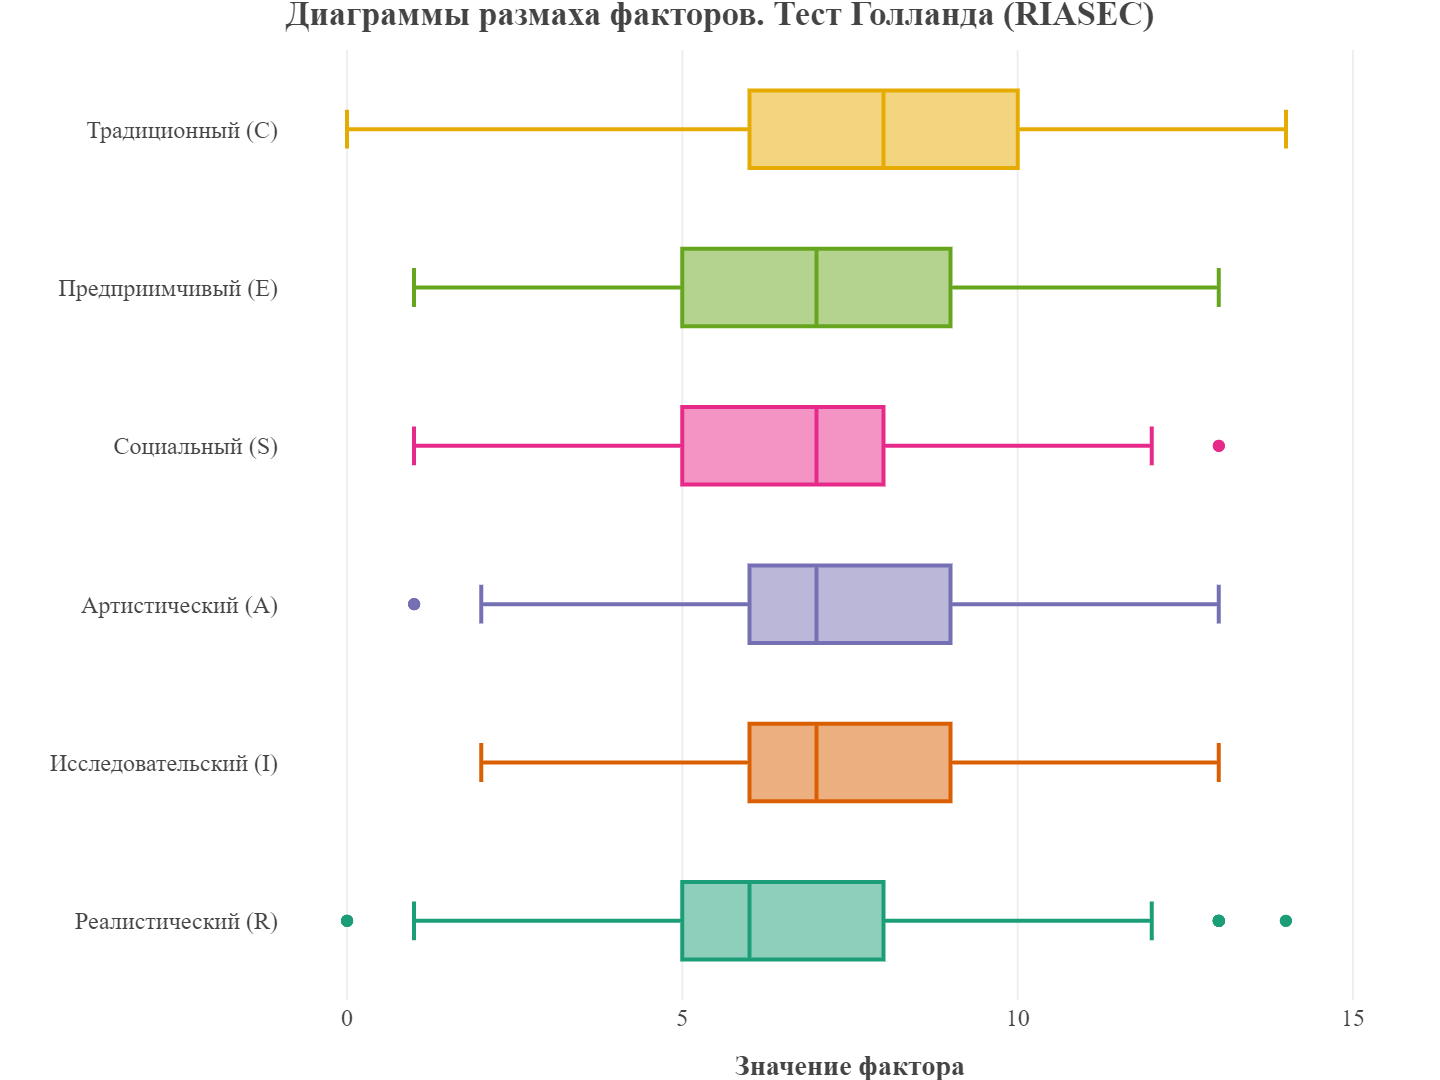
\includegraphics[width=0.85\linewidth]{figures/HL.png}
            \captionsetup{font=footnotesize}
            \caption{Диаграмма размаха факторов Голланда}
            \label{fig:HL_boxplot}
        \end{figure}
    \end{column}
    
    \end{columns}
  
    \btVFill
    {\scriptsize
        \textsuperscript{2} Мини-приложение \enquote{Психологические тесты} (\enquote{VK Mini Apps}). URL: \url{https://vk.com/app7794698}

        \textsuperscript{3} Политика конфиденциальности. URL: \url{https://vk.com/@ticslabs-politika-konfidencialnosti}
    }
\end{frame}


\begin{frame}
    \frametitle{Подходы. Базовые модели}
    \begin{itemize}
        \item Регрессия и классификация:
            \begin{itemize}
                \item модели на основе линейной регрессии (\emph{Lasso L1, Ridge L2, пошаговая})
                \item ансамбли деревьев (\emph{случайный лес, ExtraTrees})
                \item модели градиентного бустинга (\emph{CatBoost, LightGBM, XGBoost})
                \item непараметрические модели (\emph{kNN, метод опорных векторов})
                \item нейросетевые модели (\emph{MLP, TabPFN})
                \item регуляризованная логистическая регрессия (\emph{Lasso L1, Ridge L}2)
                \item наивный байесовский классификатор
                \item базовая константная модель (для сравнительного анализа)
            \end{itemize}
        \vspace{0.4em}
        \item Списочное ранжирование:
            \begin{itemize}
                \item Скоринговая функция: MLP, Deep \& Cross Network, трансформер
                \item Функции потерь: ApproxNDCG, LambdaRank, ListNet@1, ListNet@3
            \end{itemize}
    \end{itemize}
\end{frame}


\begin{frame}
    \frametitle{Сравнение регрессионных моделей}
    \renewcommand{\g}[1]{\gradientcelld{#1}{7}{10.5}{11.2}{low}{mid}{high}{70}}

\begin{table}
    \captionsetup{skip=-0.5ex, belowskip=1pt}
    \footnotesize
    \centering
    \caption{Сравнение базовых регрессионных моделей по C-индексу}
    \label{tab:regr_res}
    \setlength{\tabcolsep}{0pt}
    \begin{tabular*}{0.9\textwidth}{@{\extracolsep{\fill}}
          >{\raggedright\arraybackslash}m{5.2cm}|
          *{4}{>{\centering\arraybackslash}m{2.08cm}}
        @{}}
      \toprule
      \multicolumn{1}{>{\centering\arraybackslash}m{5.2cm}|}{\textbf{Модель}}
        & \multicolumn{2}{c}{\textbf{Multioutput}}
        & \multicolumn{2}{c}{\textbf{Chained}} \\
      \cmidrule(lr){2-3}\cmidrule(lr){4-5}
        & \textbf{без PCA} & \textbf{PCA}
        & \textbf{без PCA} & \textbf{PCA} \\
      \midrule
      Регрессия Lasso (L1)      & \g{11.175} & \g{10.887} & \g{11.175} & \g{11.150} \\
      ExtraTrees                & \g{10.700} & \g{11.100} & \g{10.625} & \g{10.825} \\
      Регрессия Ridge (L2)      & \g{10.988} & \g{10.537} & \g{11.062} & \g{10.412} \\
      Метод опорных векторов    & \g{10.713} & \g{10.950} & \g{10.713} & \g{10.950} \\
      Пошаговая регрессия       & \g{10.605} & \g{10.905} & \g{10.600} & \g{10.905} \\
      CatBoost                  & \g{10.688} & \g{10.812} & \g{10.688} & \g{10.812} \\
      Случайный лес             & \g{10.625} & \g{10.475} & \g{10.812} & \g{10.588} \\
      LightGBM                  & \g{10.750} & \g{10.425} & \g{10.750} & \g{10.425} \\
      k-ближайших соседей (kNN) & \g{10.525} & \g{10.400} & \g{10.525} & \g{10.400} \\
      XGBoost                   & \g{9.164}  & \g{9.729}  & \g{9.162}  & \g{9.725}  \\
      Базовая константная       & \g{9.000}  & \g{9.000}  & \g{9.000}  & \g{9.000}  \\
      \midrule
      TabPFN                    & \g{10.562} &            &            &            \\
      MLP (BN, DropOut, регуляризация) & \g{10.462} &     &            &            \\
      Многослойный перцептрон (MLP)    & \g{10.275} &     &            &            \\
      \bottomrule
    \end{tabular*}
    % \vspace{0.75em}
    % \begin{minipage}{\textwidth}
    %   \scriptsize
    %   \textit{\hspace*{3em} Обозначения: PCA~--- метод главных компонент (уменьшение размерности), BN~--- пакетная нормализация}
    % \end{minipage}
\end{table}


\end{frame}


\begin{frame}
    \frametitle{Сравнение подходов к классификции}
    \newcommand{\gA}[1]{\gradientcelld{#1}{0.93}{0.97}{1}{low}{mid}{high}{70}}
\newcommand{\gB}[1]{\gradientcelld{#1}{0.56}{0.69}{0.8}{low}{mid}{high}{70}}
\newcommand{\gC}[1]{\gradientcelld{#1}{0.05}{0.12}{0.23}{low}{mid}{high}{70}}


\begin{table}
  \centering
  \small
  \setlength{\tabcolsep}{0.5pt}
  \caption{Сравнение подходов к классификации (метрика Top-K accuracy)}
  \label{tab:classif_res}
  \begin{tabular*}{0.9\textwidth}{@{\extracolsep{\fill}} 
    p{3cm}|
    *{3}{>{\centering\arraybackslash}p{1.07cm}}|
    *{3}{>{\centering\arraybackslash}p{1.07cm}}|
    *{3}{>{\centering\arraybackslash}p{1.07cm}}
  @{}  }
    \toprule
    \multicolumn{1}{>{\centering\arraybackslash}p{3cm}|}{\textbf{Модель}}
      & \multicolumn{3}{c|}{\textbf{Multiclass}}
      & \multicolumn{3}{c|}{\textbf{Multilabel}}
      & \multicolumn{3}{c}{\textbf{Label Powerset}} \\
    \cmidrule(lr){2-4}\cmidrule(lr){5-7}\cmidrule(lr){8-10}
      & Top1 & Top2 & Top3 
      & Top1 & Top2 & Top3 
      & Top1 & Top2 & Top3 \\
    \midrule
    kNN                & \gA{0.99} & \gB{0.71} & \gC{0.13} & \gA{1.00} & \gB{0.76} & \gC{0.11} & \gA{0.98} & \gB{0.65} & \gC{0.18} \\
    Логистич. L1-регр. & \gA{1.00} & \gB{0.70} & \gC{0.16} & \gA{1.00} & \gB{0.70} & \gC{0.16} & \gA{0.99} & \gB{0.64} & \gC{0.10} \\
    XGBoost            & \gA{1.00} & \gB{0.70} & \gC{0.11} & \gA{0.98} & \gB{0.68} & \gC{0.10} & \gA{0.96} & \gB{0.63} & \gC{0.11} \\
    Логистич. L2-регр. & \gA{1.00} & \gB{0.70} & \gC{0.15} & \gA{0.99} & \gB{0.70} & \gC{0.21} & \gA{0.99} & \gB{0.68} & \gC{0.09} \\
    Наивный Байес      & \gA{0.98} & \gB{0.70} & \gC{0.15} & \gA{0.99} & \gB{0.70} & \gC{0.15} & \gA{0.99} & \gB{0.69} & \gC{0.16} \\
    ExtraTrees         & \gA{1.00} & \gB{0.73} & \gC{0.15} & \gA{1.00} & \gB{0.78} & \gC{0.15} & \gA{0.98} & \gB{0.69} & \gC{0.20} \\
    Метод опорн. вект. & \gA{1.00} & \gB{0.74} & \gC{0.15} & \gA{1.00} & \gB{0.72} & \gC{0.14} & \gA{0.98} & \gB{0.68} & \gC{0.21} \\
    Случайный лес      & \gA{1.00} & \gB{0.74} & \gC{0.16} & \gA{1.00} & \gB{0.74} & \gC{0.15} & \gA{0.99} & \gB{0.64} & \gC{0.23} \\
    CatBoost           & \gA{0.99} & \gB{0.79} & \gC{0.11} & \gA{0.99} & \gB{0.79} & \gC{0.11} & \gA{0.99} & \gB{0.70} & \gC{0.16} \\
    LightGBM           & \gA{0.98} & \gB{0.66} & \gC{0.09} & \gA{0.98} & \gB{0.70} & \gC{0.10} & \gA{0.95} & \gB{0.63} & \gC{0.09} \\
    \bottomrule
  \end{tabular*}
\end{table}

\end{frame}


\begin{frame}
    \frametitle{Сравнение классификационных моделей}
    \renewcommand{\g}[1]{\gradientcelld{#1}{7}{10.35}{11.3}{low}{mid}{high}{70}}
  
\begin{table}
    \setlength{\tabcolsep}{0pt}
    \small
    \centering
    \caption{Сравнение базовых классификационных моделей}
    \label{tab:best_classif}
    \begin{tabular*}{0.95\textwidth}{@{\extracolsep{\fill}}
        >{\raggedright\arraybackslash}p{5.3cm}        % Классификатор
        >{\centering\arraybackslash}p{2.25cm}          % Подход
        >{\centering\arraybackslash}p{2.25cm}        % C‑индекс
        *{3}{>{\centering\arraybackslash}p{1.25cm}}  % Top‑1,2,3
        @{}}
        \toprule
        \textbf{Классификатор}
          & \textbf{Подход}
          & \textbf{C‑индекс}
          & \textbf{Top1}
          & \textbf{Top2}
          & \textbf{Top3} \\
        \midrule
       k-ближайших соседей (kNN)    & Multilabel & \g{10.838} & 1.000 & 0.763 & 0.113 \\
        Логистическая L1-регрессия  & Multiclass & \g{10.663} & 1.000 & 0.700 & 0.163 \\
        XGBoost                     & Multiclass & \g{10.638} & 1.000 & 0.700 & 0.113 \\
        Логистическая L2-регрессия  & Multiclass & \g{10.500} & 1.000 & 0.700 & 0.150 \\
        Наивный байесовский класс-р & Multilabel & \g{10.350} & 0.988 & 0.700 & 0.150 \\
        ExtraTrees             & Multilabel & \g{10.013} & 1.000 & 0.775 & 0.146 \\
        Метод опорных векторов & Multilabel & \g{9.875}  & 1.000 & 0.721 & 0.138 \\
        Случайный лес          & Multilabel & \g{9.800}  & 0.996 & 0.738 & 0.146 \\
        CatBoost               & Multilabel & \g{9.775}  & 0.988 & 0.788 & 0.113 \\
        LightGBM               & Multilabel & \g{9.313}  & 0.975 & 0.700 & 0.100 \\
        Базовый случайный      & –          & \g{9.000}  & 0.950 & 0.500 & 0.050 \\
        \bottomrule
    \end{tabular*}
\end{table}
\end{frame}


\begin{frame}
    \frametitle{Сравнение моделей ранжирования}
    \renewcommand{\g}[1]{\gradientcelld{#1}{7}{9.6}{11.5}{low}{mid}{high}{70}}
\newcommand{\gndcg}[1]{\gradientcelld{#1}{0.25}{0.54}{0.7}{low}{mid}{high}{70}}

\begin{table}
    \setlength{\tabcolsep}{0pt}
    \small
    \centering
    \caption{Сравнение моделей ранжирования}
    \label{tab:rank}
    \begin{tabular*}{0.95\textwidth}{@{\extracolsep{\fill}} 
      >{\raggedright\arraybackslash}p{2.5cm}  % Функция потерь
      | *{3}{>{\centering\arraybackslash}m{1.9cm}}  % C‑индекс
      | *{3}{>{\centering\arraybackslash}m{1.9cm}}  % NDCG@3
    }
      \toprule
        \multicolumn{1}{c|}{\textbf{Функция}}  
          & \multicolumn{3}{c|}{\textbf{C‑индекс}} 
          & \multicolumn{3}{c}{\textbf{NDCG@3}} \\
        \cmidrule(lr){2-4} \cmidrule(lr){5-7}
        \multicolumn{1}{c|}{\textbf{потерь}}  
        & Deep\&Cross 
        & Trans\-former 
        & MLP 
        & Deep\&Cross 
        & Trans\-former 
        & MLP \\
      \midrule
      ApproxNDCG   & \g{10.025} & \g{8.888}  & \g{9.150}  & \gndcg{0.539} & \gndcg{0.439} & \gndcg{0.388} \\
      LambdaRank   & \g{9.963}  & \g{9.675}  & \g{9.650}  & \gndcg{0.527} & \gndcg{0.489} & \gndcg{0.543} \\
      ListNet@1    & \g{9.650}  & \g{10.325} & \g{10.438} & \gndcg{0.504} & \gndcg{0.628} & \gndcg{0.653} \\
      ListNet@3    & \g{9.450}  & \g{9.950}  & \g{10.788} & \gndcg{0.458} & \gndcg{0.622} & \gndcg{0.638} \\
      \bottomrule
    \end{tabular*}
\end{table}

\end{frame}


\begin{frame}
    \frametitle{Ансамблирование регрессионных моделей}
    \renewcommand{\g}[1]{\gradientcelld{#1}{9}{11.1}{11.8}{low}{mid}{high}{70}}

\begin{table}
    \captionsetup{skip=-0.5ex, belowskip=2pt}
    \footnotesize
    \setlength{\tabcolsep}{0pt}
    \caption{Сравнение методов подбора весов ансамбля регрессионных моделей}
    \label{tab:regr_ensembles}
    \begin{tabular*}{0.95\textwidth}{@{\extracolsep{\fill}}
        >{\raggedright\arraybackslash}m{5.5cm}|
        *{4}{>{\centering\arraybackslash}m{2.2cm}}
      @{}}
      \toprule
        \multicolumn{1}{>{\centering\arraybackslash}m{5.5cm}|}{\textbf{Метод подбора весов}} 
            & \multicolumn{2}{c}{\textbf{Multioutput}}
            & \multicolumn{2}{c}{\textbf{Chained}} \\
          \cmidrule(lr){2-3}\cmidrule(lr){4-5}
            & \textbf{все модели} 
            & \textbf{топ-5} 
            & \textbf{все модели} 
            & \textbf{топ-5} \\
      \midrule
      Равные веса всех моделей       & \g{11.063} & \g{11.088} & \g{11.050} & \g{11.013} \\
      Вектор Шэпли (Shap)            & \g{11.050} & \g{11.138} & \g{11.138} & \g{11.050} \\
      Частичный перебор по сетке     & \g{11.550} & \g{11.388} & \g{11.538} & \g{11.325} \\
      Квадратичная оптимизация (QP)  & \g{10.588} & \g{10.463} & \g{10.738} & \g{10.813} \\
      Генетический алгоритм (GA)     & \g{11.500} & \g{11.550} & \g{11.300} & \g{11.563} \\
      Метод роя частиц (PSO)         & \g{11.600} & \g{11.663} & \g{11.613} & \g{11.613} \\
      Координатный спуск             & \g{11.188} & \g{11.225} & \g{11.288} & \g{11.413} \\
      \midrule
      Лин. регрессии с регуляризацией 
        & \multicolumn{2}{c}{Линейная регрессия} 
        & \multicolumn{2}{c}{\g{10.887}} \\
      L1, L2, LightGBM, CatBoost, RF 
        & \multicolumn{2}{c}{Линейная регрессия} 
        & \multicolumn{2}{c}{\g{10.688}} \\
      \bottomrule
    \end{tabular*}
    % \begin{minipage}{\textwidth}
    %   \footnotesize
    %   \textit{\hspace*{1.5em}Обозначения:\\
    %   \hspace*{2.5em}топ-5~--- подбор весов только для топ-5 моделей по C-индексу\\
    %   \hspace*{2.5em}L1 и L2~--- Lasso- и Ridge-модели регрессии, RF~--- случайный лес}
    % \end{minipage}
\end{table}

    % \begin{table}
%     \setlength{\tabcolsep}{0pt}
%     \centering
%     \caption{Весовые коэффициенты моделей и C-индекс для PSO}
%     \label{tab:pso_regr_weights}
%     \begin{tabular*}{\textwidth}{@{\extracolsep{\fill}} 
%         l*{4}{c}>{\centering\arraybackslash}p{1.3cm}
%         >{\raggedright\arraybackslash}p{1.3cm}@{}}
%         \toprule
%         \textbf{Подбор} & \multicolumn{4}{c}{\textbf{Веса моделей}} & \textbf{\quad C-} \\
%         \cmidrule(lr){2-5}
%         \textbf{весов} & Lasso L1 & Пошаговая регр. & CatBoost & ExtraTrees & \textbf{индекс} \\
%         \midrule
%         PSO & 0.432 & 0.327 & 0.150 & 0.091 & 11.663 \\
%         \bottomrule
%     \end{tabular*}
% \end{table}

\begin{table}
    \captionsetup{skip=-1ex, belowskip=0pt}
    \centering
    \footnotesize
    % \caption{Весовые коэффициенты моделей PSO-ансамбля подхода Multioutput}
    \label{tab:pso_regr_weights}
    \setlength{\tabcolsep}{4pt}
    \begin{tabular*}{0.95\textwidth}{@{\extracolsep{\fill}}
          >{\raggedright\arraybackslash}p{3.5cm}|
          *{4}{>{\centering\arraybackslash}c}|c
        @{}}
      \toprule
      \textbf{Подбор весов}
        & \textbf{Lasso L1}
        & \textbf{Пошаговая регр.}
        & \textbf{CatBoost}
        & \textbf{ExtraTrees} & \textbf{\Large$\Sigma$} \\
      \midrule
      PSO, топ-5 multioutput & 0.432 & 0.327 & 0.150 & 0.091 & = 1.000 \\
      \bottomrule
    \end{tabular*}
\end{table}


\end{frame}


\begin{frame}
    \frametitle{Ансамблирование классификационных моделей}
    \renewcommand{\g}[1]{\gradientcelld{#1}{8}{10.8}{11.7}{low}{mid}{high}{70}}

\begin{table}
    \captionsetup{skip=-0.5ex, belowskip=1pt}
    \small
    \setlength{\tabcolsep}{0pt}
    \centering
    \caption{Сравнение методов подбора весов ансамбля классификаторов}
    \label{tab:clsf_ensemble}
    \begin{tabular*}{0.9\textwidth}{@{\extracolsep{\fill}}
        >{\raggedright\arraybackslash}m{5.5cm}|
        *{3}{>{\centering\arraybackslash}m{2.65cm}} @{}}
        \toprule
        \multicolumn{1}{c|}{\textbf{Метод подбора весов}}
          & \textbf{Multiclass}
          & \textbf{Multilabel}
          & \textbf{Label Powerset} \\
        \midrule
        Равные веса всех моделей      & \g{10.663} & \g{10.888} & \g{10.563} \\
        Вектор Шэпли (Shap)           & \g{10.563} & \g{11.038} & \g{10.525} \\
        Частичный перебор по сетке    & \g{11.213} & \g{11.488} & \g{11.525} \\
        Квадратичная оптимизация (QP) & \g{10.488} & \g{10.638} & \g{10.650} \\
        Генетический алгоритм (GA)    & \g{11.263} & \g{11.313} & \g{11.213} \\
        Метод роя частиц (PSO)        & \g{11.263} & \g{11.625} & \g{11.525} \\
        Координатный спуск            & \g{11.200} & \g{11.275} & \g{10.425} \\
        \bottomrule
    \end{tabular*}
\end{table}

    % \begin{table}
%     \setlength{\tabcolsep}{0pt}
%     \centering
%     \caption{Весовые коэффициенты моделей и C‑индекс для PSO}
%     \label{tab:clsf_pso_w}
%     \begin{tabular*}{\textwidth}{@{\extracolsep{\fill}} 
%           >{\centering\arraybackslash}p{1.5cm}
%           *{5}{c}>{\centering\arraybackslash}p{1.3cm}
%           >{\raggedright\arraybackslash}p{1.2cm}
%         @{}}
%           \toprule
%           \textbf{Подбор} & \multicolumn{5}{c}{\textbf{Веса моделей}} & \textbf{\quad C-}\\
%           \cmidrule(lr){2-6}
%           \textbf{весов} & kNN & SVM & Logit L1 & XGBoost & LightGBM & \textbf{индекс}\\
%           \midrule
%           PSO & 0.291 & 0.164 & 0.191 & 0.183 & 0.151 & 11.625 \\
%           \bottomrule
%     \end{tabular*}
% \end{table}

\begin{table}
    \captionsetup{skip=-0.5ex, belowskip=1pt}
    \centering
    \small
    \caption{Весовые коэффициенты моделей для PSO}
    \label{tab:clsf_pso_w}
    \setlength{\tabcolsep}{4pt}
    \begin{tabular*}{0.9\textwidth}{@{\extracolsep{\fill}}
          >{\raggedright\arraybackslash}p{2.5cm}|
          *{6}c|c
        @{}}
      \toprule
      \textbf{Подбор весов} & \textbf{kNN} & \textbf{Logit L1} & \textbf{XGBoost} & \textbf{SVM} & \textbf{LightGBM} & \textbf{$\cdots$} & \textbf{\Large$\Sigma$}\\
      \midrule
      PSO & 0.291 & 0.191 & 0.183 & 0.164 & 0.151 & 0.020 & = 1.000\\
      \bottomrule
    \end{tabular*}
\end{table}

\end{frame}


\begin{frame}
    \frametitle{Методы восстановления результатов незаполненных тестов}
    \renewcommand{\g}[1]{\gradientcelld{#1}{7}{9.6}{10.5}{low}{mid}{high}{70}}
  
\begin{table}
    \captionsetup{skip=-0.5ex, belowskip=1pt}
    \setlength{\tabcolsep}{0pt}
    \small
    \centering
    \caption{Восстановление значений незаполненных психометрических тестов с помощью базовых регрессионных моделей}
    \label{tab:impute}
        \begin{tabular*}{0.9\textwidth}{@{\extracolsep{\fill}} 
        >{\raggedright\arraybackslash}m{5cm}|
        *{4}{>{\centering\arraybackslash}m{2.15cm}}
        @{}}
        \toprule
        \multicolumn{1}{c|}{\textbf{Модель-регрессор}} & 
        \textbf{MICE} & \textbf{Soft Impute} & \textbf{Маски} & \textbf{Ансам\-бли} \\
        \midrule
        Регрессия Lasso (L1)   & \g{9.191} & \g{10.248}  & \g{9.998} & \g{9.866} \\
        Пошаговая регрессия    & \g{9.608} & \g{10.183}  & \g{9.978} & \g{10.082}\\
        Случайный лес          & \g{9.518} & \g{10.136}  & \g{9.819} & \g{9.712} \\
        LightGBM               & \g{9.372} & \g{10.086}  & \g{9.686} & \g{9.594} \\
        Линейная регрессия (OLS) & \g{9.407} & \g{10.021}  & \g{9.876} & \g{10.012}\\
        Регрессия Ridge (L2)   & \g{9.442} & \g{9.770}   & \g{9.868} & \g{9.933} \\
        ExtraTrees             & \g{9.101} & \g{9.823}   & \g{9.870} & \g{9.808} \\
        Метод опорных векторов & \g{9.221} & \g{9.814}   & \g{9.864} & \g{9.760} \\
        CatBoost               & \g{9.131} & \g{9.814}   & \g{9.835} & \g{9.461} \\
        k-ближайших соседей (kNN) & \g{9.372} & \g{9.834}   & \g{9.830} & \g{9.377} \\
        XGBoost                & \g{8.769} & \g{9.571}   & \g{9.267} & \g{9.614} \\
        Базовая константная    & \g{9.000} & \g{9.000}   & \g{9.000} & \g{9.000} \\
        \bottomrule
    \end{tabular*}
\end{table}
\end{frame}


\begin{frame}
    \frametitle{Ансамблевые методы восстановления для Soft Impute}
    \renewcommand{\g}[1]{\gradientcelld{#1}{9}{10.25}{11}{low}{mid}{high}{70}}

\begin{table}
    \footnotesize
    \setlength{\tabcolsep}{0pt}
    \centering
    \caption{Весовые коэффициенты моделей и C-индекс при разных методах подбора весов для ансамблей на восстановленных данных}
    \label{tab:impute_ens}
    \begin{tabular*}{0.95\textwidth}{@{\extracolsep{\fill}} 
        >{\raggedright\arraybackslash}m{4.35cm}|
        *{5}{>{\centering\arraybackslash}m{1.5cm}}|
        >{\centering\arraybackslash}m{2cm}
      @{}}
        \toprule
        \multicolumn{1}{c|}{\textbf{Подбор весов}} 
          & \multicolumn{5}{c|}{\textbf{Веса моделей}} 
          & \textbf{С-индекс}\\
        \cmidrule(lr){2-6}
        \multicolumn{1}{c|}{}  
          & \textbf{Lasso L1} 
          & \textbf{Пошагов.} 
          & \textbf{LightGBM} 
          & \textbf{Случ. лес} 
          & \textbf{kNN} 
          & \textbf{} \\
        \midrule
        Метод роя частиц (PSO)     & 0.001 & 0.481 & 0.038 & 0.475 & 0.005 & \g{10.740} \\
        Частичный перебор по сетке & 0.000 & 0.500 & 0.000 & 0.500 & 0.000 & \g{10.657} \\
        Генетический алгоритм (GA) & 0.281 & 0.369 & 0.109 & 0.189 & 0.052 & \g{10.401} \\
        Координатный спуск         & 0.019 & 0.422 & 0.067 & 0.305 & 0.187 & \g{10.245} \\
        Квадратичная оптимиз. (QP) & 0.050 & 0.000 & 0.390 & 0.007 & 0.553 & \g{10.065} \\
        Равные веса всех моделей   & 0.200 & 0.200 & 0.200 & 0.200 & 0.200 & \g{10.053} \\
        Вектор Шэпли (Shap)        & 0.247 & 0.185 & 0.206 & 0.179 & 0.183 & \g{10.047} \\
        \bottomrule
    \end{tabular*}
        \vspace{0.5em}
        \begin{minipage}{\textwidth}
        \scriptsize
        \textit{\hspace*{1.5em}Обозначения:\\
        \hspace*{2.5em}Пошагов. ~--- пошаговая регрессия,\\
        \hspace*{2.5em}Случ. лес~--- случайный лес (Random Forest),\\
        \hspace*{2.5em}kNN~--- метод k-ближайших соседей}
    \end{minipage}
\end{table}

\end{frame}


\begin{frame}
    \frametitle{Итоговая последовательность вычислительных шагов}
    
    \begin{figure}
        \centering
        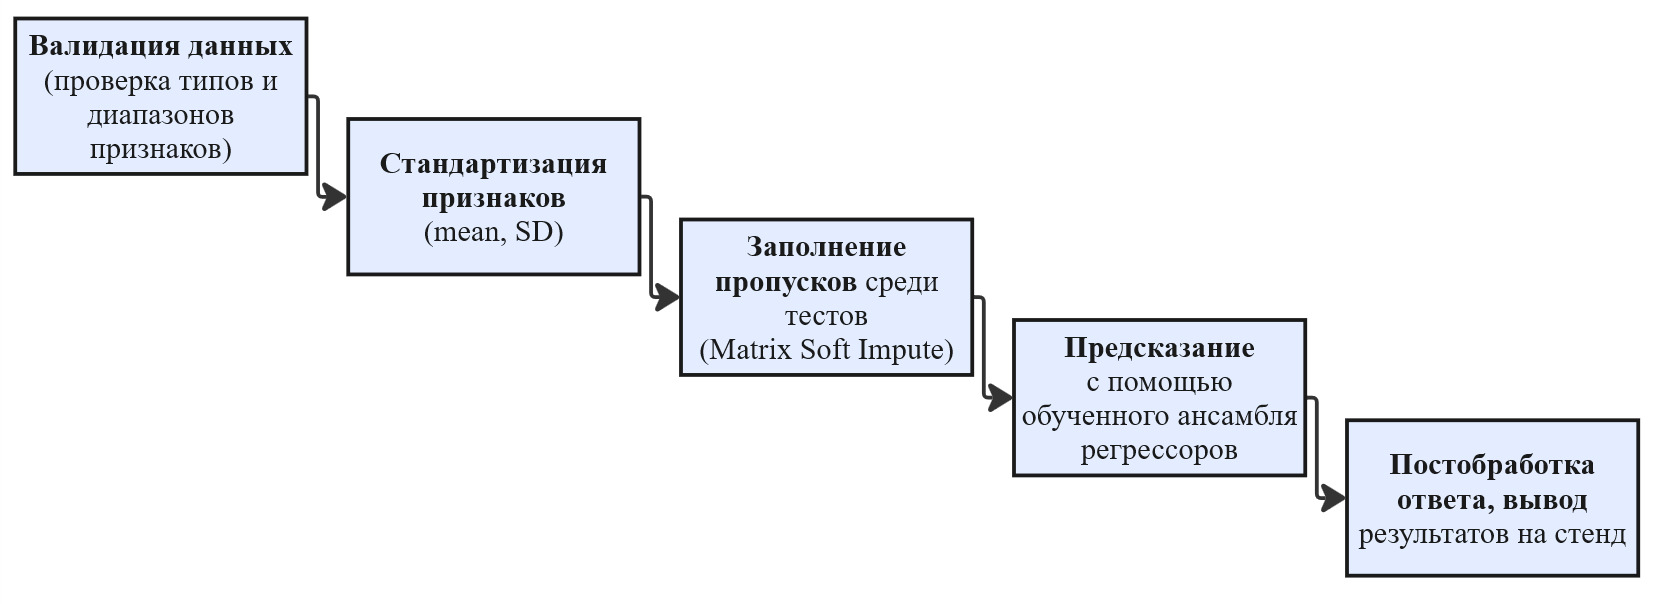
\includegraphics[width=0.95\linewidth]{figures/final_pipeline.jpg}
        \caption{Итоговая последовательность шагов вычислительного конвейера\textsuperscript{4}}
        \label{fig:pipeline}
    \end{figure}


    \btVFill
    {\footnotesize \quad
        \textsuperscript{4} Предсказание кода Голланда по результатам психометрических тестов~--- Shinyapps.io\\
        \qquad URL: \url{https://exp98.shinyapps.io/diploma_holland} (дата обращения: 07.06.2025)
    }
\end{frame}


\begin{frame}
    \frametitle{Интерфейс прототипа инструмента профориентации}
    \begin{figure}
        \centering
        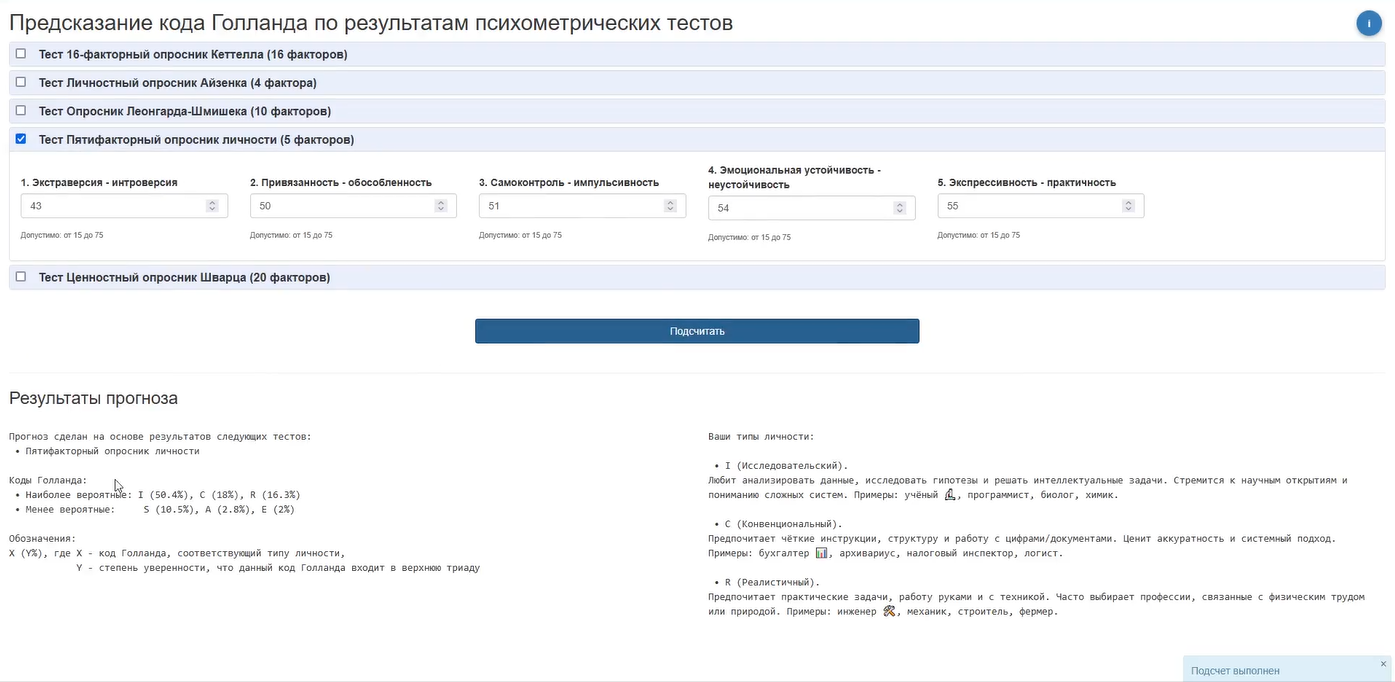
\includegraphics[width=1.0\linewidth]{figures/UI2.png}
        \caption{Интерфейс прототипа инструмента профориентации}
        \label{fig:ui2}
    \end{figure}
\end{frame}


\begin{frame}
    \frametitle{Результаты экспериментов}
    \begin{itemize}
        \item Лучшая базовая модель~--- L1-регрессия с независимыми выходами:\\$C_{index}~=~11.175$
        
        \vspace{0.5em}
        \item Превосходство классических методов машинного обучения над нейросетевыми~--- лучшая среди нейронных сетей MLP (ListNet@3): $C_{index}~=~10.788$

        \vspace{0.5em}
        \item Ансамблевые модели (подбор весов методом роя частиц): 
        \begin{itemize}
            \item ансамбль регрессоров с независимыми выходами: $C_{index}~=~11.663$
            \item ансамбль классификаторов со многими метками: $C_{index}~=~11.625$
        \end{itemize}

        \vspace{0.5em}
        \item Для восстановления данных предпочтителен метод мягкой импутации\\\emph{Soft Impute}: $C_{index}~=~10.740$
    \end{itemize}
\end{frame}


\begin{frame}
    \frametitle{Результаты}
    \begin{enumerate}
        \item Реализованы\textsuperscript{5} подходы к определению кода Голланда: регрессия, классификация, списочное ранжирование
        \item Разработан модуль формирования взвешенного ансамбля моделей
        \item Проведен сравнительный анализ моделей предсказания кодов Голланда
        \item Разработаны и реализованы математические модели модуля восстановления пропусков результатов психометрических тестов
        \item Создан прототип инструмента для определения профориентационных предпочтений на основе R Shiny
        \vspace{0.8em}
        \item[$\circ$] Участие в XXVIII Международной конференции SCM'25
        \item[$\circ$] Акт об использовании результатов ВКР в НИР СПб ФИЦ РАН
    \end{enumerate}

    \btVFill
    {\footnotesize
        \textsuperscript{5} GitHub: Предсказание кода Голланда (RIASEC) по результатам психометрических тестов личности.\\\quad URL: \url{https://github.com/ExP98/Diploma_Holland} (дата обращения: 07.06.2025)\\
    }
\end{frame}


%\addtocounter{framenumber}{1}
\appendix

\begin{frame}{Акт об использовании результатов ВКР}
  \begin{columns}[T,onlytextwidth]
    \column{0.48\textwidth}
      \centering
      
\includegraphics[width=0.72\linewidth]{figures/Акт-1.PNG}
    \column{0.48\textwidth}
      \centering
      
\includegraphics[width=0.75\linewidth]{figures/Акт-2.PNG}
  \end{columns}
\end{frame}


\begin{frame}
    \frametitle{Ссылки на дополнительные материалы}
    \begin{itemize}
        \item Исходный код\textsuperscript{1}
        \item Веб-приложение\textsuperscript{2}
        \item Участие в XXVIII Международной конференции по мягким вычислениям и измерениям SCM'25\textsuperscript{3}
    \end{itemize}
    
    \btVFill
    {\footnotesize
        \textsuperscript{1} GitHub: Предсказание кода Голланда (RIASEC) по результатам психометрических тестов личности. URL: \url{https://github.com/ExP98/Diploma_Holland} (дата обращения: 07.06.2025)\\
        \vspace{0.2em}
        \textsuperscript{2} Предсказание кода Голланда по результатам психометрических тестов - Shinyapps.io. URL: \url{https://exp98.shinyapps.io/diploma_holland} (дата обращения: 07.06.2025)\\
        \vspace{0.2em}
        \textsuperscript{3} Тенденции взаимосвязи личностных особенностей и результатов теста Голланда среди пользователей социальной сети ВКонтакте. URL: \url{https://scm.etu.ru/assets/files/2025/sbornik/044-048.pdf} (дата обращения: 07.06.2025)
    }
\end{frame}


\begin{frame}
    \frametitle{Анализ важности признаков}
    \begin{table}
    \captionsetup{skip=-1ex, belowskip=1pt}
  \centering
  \small
  \caption{Усредненная оценка важности признаков модели случайного леса}
  \label{tab:feature_imp}
  \begin{tabular*}{0.9\textwidth}{@{\extracolsep{\fill}} 
      >{\centering\arraybackslash}p{2cm}|
      >{\raggedright\arraybackslash}p{6cm}|
      >{\centering\arraybackslash}p{2.2cm}|
      >{\centering\arraybackslash}p{2.2cm} @{}}
    \toprule
    \makecell{\textbf{Код}\\\textbf{признака}} 
      & \makecell[c]{\textbf{Наименование признака}} 
      & \makecell{\textbf{Важность}\\\textbf{(\%)}} 
      & \makecell{\textbf{Накоплено}\\\textbf{(\%)}} \\
    \midrule
    CT\_1   & Открытость--замкнутость                & 15.5 & 15.5 \\
    CT\_7   & Чувственность--твердость               & 15.5 & 31.0 \\
    SC\_19  & Гедонизм--индивидуальный приоритет     & 4.2  & 35.2 \\
    EY\_1   & Экстраверсия                           & 4.0  & 39.2 \\
    CT\_4   & Беспечность--озабоченность             & 3.6  & 42.8 \\
    SC\_3   & Власть--нормативный идеал              & 3.4  & 46.2 \\
    LN\_3   & Циклотимность                          & 3.3  & 49.5 \\
    BF\_3   & Самоконтроль--импульсивность           & 2.5  & 52.0 \\
    \bottomrule
  \end{tabular*}
\end{table}
    \begin{itemize}
        \item Два наиболее важных признака (Кеттелла)~--- более 30\% накопленной важности
        \item Первые восемь признаков~--- более 50\% (всего 55 признаков)
    \end{itemize}
\end{frame}


\begin{frame}
    \frametitle{Распределение значений C-индекса для предсказаний}
    \begin{figure}
        \centering
        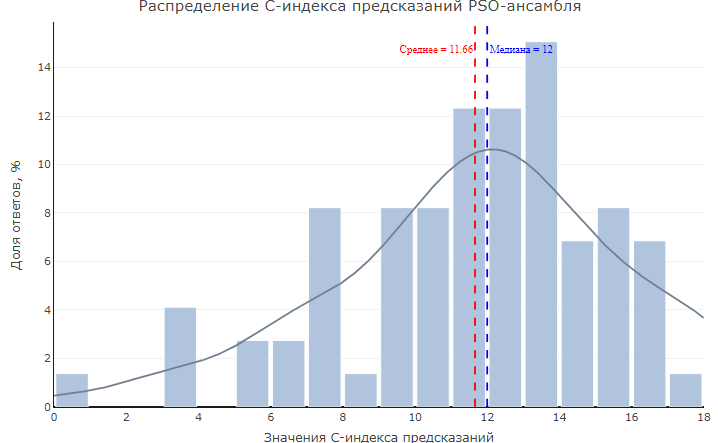
\includegraphics[width=0.65\linewidth]{figures/Cindex_distr_PSO_regr.png}
        \caption{Распределение значений C-индекса для предсказаний PSO-ансамбля регрессоров}
        \label{fig:cindex_distr}
    \end{figure}
\end{frame}


\begin{frame}
    \frametitle{Обзор лучших моделей для каждого типа задач}
    \renewcommand{\g}[1]{\gradientcelld{#1}{10}{10.65}{11.7}{low}{mid}{high}{60}}

\begin{table}
    \footnotesize
    \captionsetup{skip=0ex, belowskip=2pt}
    \setlength{\tabcolsep}{2pt}
    \centering
    \caption{Обзор лучших моделей для каждого подхода и типа задач}
    \label{tab:summary}
    \begin{tabular*}{0.95\textwidth}{@{\extracolsep{\fill}}
            >{\raggedright\arraybackslash}m{2.43cm}  % Тип задач
          | >{\raggedright\arraybackslash}m{2.43cm}  % Подход
          | >{\raggedright\arraybackslash}m{6.2cm}   % Лучшая модель
          | >{\centering\arraybackslash}m{2.85cm}       % C‑индекс
        @{}}
        \toprule
        \multicolumn{1}{c|}{\textbf{Тип задач}}
          & \multicolumn{1}{c|}{\textbf{Подход}}
          & \multicolumn{1}{c|}{\textbf{Лучшая модель}}
          & \multicolumn{1}{c}{\textbf{C-индекс}} \\
        \specialrule{0.2pt}{1pt}{1pt}
        Регрессия       & ансамбль, mo
                        & Рой частиц (Lasso-регрессия, пошаговая регрессия, CatBoost, ExtraTrees)
                        & \g{11.663} \\
        \specialrule{0.2pt}{1pt}{1pt}
        Классификация   & ансамбль, ml
                        & Рой частиц (kNN, SVM, логистическая Lasso-регрессия, XGBoost, LightGBM и др.)
                        & \g{11.625} \\
        \specialrule{0.2pt}{1pt}{1pt}
        Регрессия       & ансамбль, chain
                        & Рой частиц
                        & \g{11.613} \\
        \specialrule{0.2pt}{1pt}{1pt}
        Классификация   & ансамбль, lp
                        & Рой частиц / поиск по сетке
                        & \g{11.525} \\
        \specialrule{0.2pt}{1pt}{1pt}
        Классификация   & ансамбль, mc
                        & Генетический алгоритм / Рой частиц
                        & \g{11.263} \\
        \specialrule{0.2pt}{1pt}{1pt}
        Регрессия       & multioutput
                        & Lasso-регрессия
                        & \g{11.175} \\
        \specialrule{0.2pt}{1pt}{1pt}
        Регрессия       & chained
                        & Ridge-регрессия
                        & \g{11.062} \\
        \specialrule{0.2pt}{1pt}{1pt}
        Классификация   & multilabel
                        & k-ближайших соседей (kNN)
                        & \g{10.838} \\
        \specialrule{0.2pt}{1pt}{1pt}
        Ранжирование    & списочное
                        & MLP с ListNet@3
                        & \g{10.788} \\
        \specialrule{0.2pt}{1pt}{1pt}
        Классификация   & multiclass
                        & Логистическая Lasso-регрессия
                        & \g{10.663} \\
        \bottomrule
    \end{tabular*}
    \begin{minipage}{\textwidth}
      \scriptsize
      \textit{\hspace*{1.5em}Обозначения: mo~--- multioutput, ml~--- multilabel, lp~--- label powerset, mc~--- multiclass,\\
      \hspace*{2em}MLP~--- многослойный перцептрон, SVM~--- метод опорных векторов, kNN~--- метод k-ближайших соседей}
    \end{minipage}
\end{table}
\end{frame}


\begin{frame}
    \frametitle{Метрики качества RMSE и NDCG}
    \begin{itemize}
    \item Корень из среднеквадратичной ошибки (RMSE):
      \[
        \mathrm{RMSE}
        = \sqrt{\frac{1}{n}\sum_{i=1}^n \bigl(y_i - \hat{y}_i\bigr)^2},
      \]
      где \(n\)~--- число объектов, \(y_i\) и \(\hat{y}_i\)~--- истинное и предсказанное значения

    \vspace{0.2em}
    \item Нормализованный дисконтированный совокупный прирост (NDCG@K):
    \begin{flalign*}
        \mathrm{DCG@K} = \sum_{i=1}^K \frac{2^{\mathrm{rel}_i}-1}{\log_2(i+1)}, \;
        \mathrm{IDCG@K} = \sum_{i=1}^K \frac{2^{\mathrm{rel}_i^\ast}-1}{\log_2(i+1)}, \;
        \mathrm{NDCG@K} = \frac{\mathrm{DCG@K}}{\mathrm{IDCG@K}},&&
    \end{flalign*}
    где \(K\) — глубина ранжирования, \(\mathrm{rel}_i\) и \(\mathrm{rel}_i^*\)~--- релевантность i-го элемента в ранжированном списке и в идеальном ранжировании
    \end{itemize}
\end{frame}


\begin{frame}
    \frametitle{Сравнение регрессионных моделей (RMSE)}
    \renewcommand{\gr}[1]{\gradientcelld{#1}{2.01}{2.1}{2.8}{high}{mid}{low}{70}}

\begin{table}
    \captionsetup{skip=-0.5ex, belowskip=2pt}
    \footnotesize
    \centering
    \caption{Сравнение базовых регрессионных моделей по RMSE}
    \label{tab:rmse-comparison}
    \setlength{\tabcolsep}{2pt}
    \begin{tabular*}{0.9\textwidth}{@{\extracolsep{\fill}}
          >{\raggedright\arraybackslash}m{5cm}|
          *{4}{>{\centering\arraybackslash}m{2cm}}
        @{}}
      \toprule
      \multicolumn{1}{>{\centering\arraybackslash}m{5cm}|}{\textbf{Имя}}
        & \multicolumn{2}{c}{\textbf{Multioutput}}
        & \multicolumn{2}{c}{\textbf{Chained}} \\
      \cmidrule(lr){2-3}\cmidrule(lr){4-5}
        & \textbf{без PCA} & \textbf{PCA}
        & \textbf{без PCA} & \textbf{PCA} \\
      \midrule
      Регрессия Lasso (L1)         & \gr{2.018} & \gr{2.036} & \gr{2.018} & \gr{2.030} \\
      Регрессия Ridge (L2)         & \gr{2.025} & \gr{2.037} & \gr{2.028} & \gr{2.044} \\
      Пошаговая регрессия          & \gr{2.094} & \gr{2.027} & \gr{2.094} & \gr{2.027} \\
      CatBoost                     & \gr{2.044} & \gr{2.096} & \gr{2.044} & \gr{2.096} \\
      Случайный лес                & \gr{2.069} & \gr{2.131} & \gr{2.070} & \gr{2.133} \\
      LightGBM                     & \gr{2.074} & \gr{2.128} & \gr{2.074} & \gr{2.128} \\
      Метод опорных векторов (SVR) & \gr{2.100} & \gr{2.101} & \gr{2.100} & \gr{2.101} \\
      ExtraTrees                   & \gr{2.100} & \gr{2.150} & \gr{2.112} & \gr{2.152} \\
      k-ближайших соседей (kNN)    & \gr{2.162} & \gr{2.151} & \gr{2.162} & \gr{2.151} \\
      Базовая константная          & \gr{2.308} & \gr{2.308} & \gr{2.308} & \gr{2.308} \\
      XGBoost                      & \gr{2.317} & \gr{2.314} & \gr{2.317} & \gr{2.314} \\
      \midrule
      TabPFN                            & \gr{2.056} & & & \\
      MLP (BN, DropOut, регуляризация)  & \gr{2.143} & & & \\
      MLP                               & \gr{2.442} & & & \\
      \bottomrule
    \end{tabular*}
    % \vspace{0.75em}
    % \begin{minipage}{\textwidth}
    %   \scriptsize
    %   \textit{\hspace*{3em}Обозначения: PCA~--- метод главных компонент (уменьшение размерности), BN~--- пакетная нормализация}
    % \end{minipage}
\end{table}

\end{frame}

\begin{frame}
    \frametitle{Результаты ансамбля регрессионных моделей (RMSE)}
    \renewcommand{\gr}[1]{\gradientcelld{#1}{2.025}{2.05}{2.2}{high}{mid}{low}{70}}

\begin{table}
    \captionsetup{skip=-0.5ex, belowskip=2pt}
    \centering
    \small
    \setlength{\tabcolsep}{0pt}
    \caption{Сравнение методов подбора весов ансамбля регрессионных моделей по RMSE}
    \label{tab:regr_ensembles_rmse}
    \begin{tabular*}{0.95\textwidth}{@{\extracolsep{\fill}}
        >{\raggedright\arraybackslash}m{5.5cm}|
        *{4}{>{\centering\arraybackslash}m{2.2cm}}
      @{}}
      \toprule
        \multicolumn{1}{>{\centering\arraybackslash}m{5.5cm}|}{\textbf{Метод подбора весов}}
          & \multicolumn{2}{c}{\textbf{Multioutput}}
          & \multicolumn{2}{c}{\textbf{Chained}} \\
        \cmidrule(lr){2-3}\cmidrule(lr){4-5}
          & \textbf{все модели} & \textbf{топ-5}
          & \textbf{все модели} & \textbf{топ-5} \\
      \midrule
      Равные веса всех моделей        & \gr{2.052} & \gr{2.038} & \gr{2.052} & \gr{2.032} \\
      Вектор Шэпли (Shap)             & \gr{2.047} & \gr{2.035} & \gr{2.046} & \gr{2.033} \\
      Частичный перебор по сетке      & \gr{2.052} & \gr{2.026} & \gr{2.045} & \gr{2.035} \\
      Квадратичная оптимизация (QP)   & \gr{2.109} & \gr{2.093} & \gr{2.111} & \gr{2.070} \\
      Генетический алгоритм (GA)      & \gr{2.035} & \gr{2.036} & \gr{2.044} & \gr{2.032} \\
      Метод роя частиц (PSO)          & \gr{2.049} & \gr{2.031} & \gr{2.065} & \gr{2.026} \\
      Координатный спуск              & \gr{2.097} & \gr{2.048} & \gr{2.089} & \gr{2.040} \\
      \midrule
      Лин. регрессии с регуляризацией
        & \multicolumn{2}{c}{Линейная регрессия}
        & \multicolumn{2}{c}{\gr{2.111}} \\
      L1, L2, LightGBM, CatBoost, RF
        & \multicolumn{2}{c}{Линейная регрессия}
        & \multicolumn{2}{c}{\gr{2.091}} \\
      \bottomrule
    \end{tabular*}
    \begin{minipage}{\textwidth}
      \footnotesize
      \textit{\hspace*{1.5em}Обозначения:\\
      \hspace*{2.5em}топ-5~--- подбор весов только для топ-5 моделей согласно метрике,\\
      \hspace*{2.5em}L1 и L2~--- Lasso- и Ridge-модели регрессии, RF~--- случайный лес}
    \end{minipage}
\end{table}

\end{frame}


\begin{frame}
    \frametitle{Методы восстановления данных (RMSE)}
    \renewcommand{\gr}[1]{\gradientcelld{#1}{2.045}{2.1}{2.3}{high}{mid}{low}{70}}

\begin{table}
    \setlength{\tabcolsep}{0pt}
    \small
    \centering
    \caption{Восстановление значений незаполненных психометрических тестов с помощью базовых регрессионных моделей (RMSE)}
    \label{tab:impute_rmse}
    \begin{tabular*}{0.9\textwidth}{@{\extracolsep{\fill}} 
        >{\raggedright\arraybackslash}m{6cm}|
        *{3}{>{\centering\arraybackslash}m{2.5cm}}
      @{}}
        \toprule
        \multicolumn{1}{c|}{\textbf{Модель-регрессор}} 
          & \textbf{MICE} 
          & \textbf{Soft Impute} 
          & \textbf{Маски} \\
        \midrule
        Регрессия Lasso (L1)            & \gr{2.059} & \gr{2.046} & \gr{2.098} \\
        CatBoost                        & \gr{2.054} & \gr{2.092} & \gr{2.105} \\
        Пошаговая регрессия             & \gr{2.118} & \gr{2.059} & \gr{2.154} \\
        Линейная регрессия (OLS)        & \gr{2.126} & \gr{2.065} & \gr{2.174} \\
        Регрессия Ridge (L2)            & \gr{2.068} & \gr{2.125} & \gr{2.101} \\
        Случайный лес                   & \gr{2.081} & \gr{2.085} & \gr{2.113} \\
        ExtraTrees                      & \gr{2.083} & \gr{2.126} & \gr{2.133} \\
        LightGBM                        & \gr{2.083} & \gr{2.110} & \gr{2.136} \\
        Метод опорных векторов (SVR)    & \gr{2.127} & \gr{2.154} & \gr{2.105} \\
        k-ближайших соседей (kNN)       & \gr{2.107} & \gr{2.150} & \gr{2.142} \\
        Базовая константная             & \gr{2.203} & \gr{2.247} & \gr{2.244} \\
        XGBoost                         & \gr{2.212} & \gr{2.261} & \gr{2.238} \\
        \bottomrule
    \end{tabular*}
\end{table}


\end{frame}

\begin{frame}
    \frametitle{Ансамблевые методы восстановления для Soft Impute (RMSE)}
    \renewcommand{\gr}[1]{\gradientcelld{#1}{2.038}{2.06}{2.14}{high}{mid}{low}{70}}

\begin{table}
    \captionsetup{skip=-0.5ex, belowskip=2pt}
    \footnotesize
    \setlength{\tabcolsep}{0pt}
    \centering
    \caption{Весовые коэффициенты моделей и RMSE при разных методах подбора весов для ансамблей на восстановленных данных}
    \label{tab:impute_ens_rmse}
    \begin{tabular*}{0.95\textwidth}{@{\extracolsep{\fill}}
        >{\raggedright\arraybackslash}m{4.35cm}|
        *{5}{>{\centering\arraybackslash}m{1.51cm}}
        |>{\centering\arraybackslash}m{1.9cm}
      @{}}
      \toprule
      \multicolumn{1}{c|}{\textbf{Подбор весов}}
        & \multicolumn{5}{c|}{\textbf{Веса моделей}}
        & \textbf{RMSE} \\
      \cmidrule(lr){2-6}
      \multicolumn{1}{c|}{}
        & \textbf{Lasso L1}
        & \textbf{Пошагов.}
        & \textbf{LightGBM}
        & \textbf{Случ. лес}
        & \textbf{kNN}
        & \\ 
      \midrule
      Метод роя частиц (PSO)     & 0.001 & 0.481 & 0.038 & 0.475 & 0.005 & \gr{2.038} \\
      Частичный перебор по сетке & 0.000 & 0.500 & 0.000 & 0.500 & 0.000 & \gr{2.043} \\
      Генетический алгоритм (GA) & 0.281 & 0.369 & 0.109 & 0.189 & 0.052 & \gr{2.044} \\
      Координатный спуск         & 0.019 & 0.422 & 0.067 & 0.305 & 0.187 & \gr{2.052} \\
      Вектор Шэпли (Shap)        & 0.247 & 0.185 & 0.206 & 0.179 & 0.183 & \gr{2.063} \\
      Равные веса всех моделей   & 0.200 & 0.200 & 0.200 & 0.200 & 0.200 & \gr{2.064} \\
      Квадратичная оптимиз. (QP) & 0.050 & 0.000 & 0.390 & 0.007 & 0.553 & \gr{2.114} \\
      \bottomrule
    \end{tabular*}
    \vspace{0.5em}
    \begin{minipage}{\textwidth}
      \scriptsize
      \textit{\hspace*{1.5em}Обозначения:\\
      \hspace*{2.5em}Пошагов.~--- пошаговая регрессия,\\
      \hspace*{2.5em}Случ. лес~--- случайный лес (Random Forest),\\
      \hspace*{2.5em}kNN~--- метод k-ближайших соседей}
    \end{minipage}
\end{table}

\end{frame}

\end{document}
